% =========================================================================
%  CSE 625 - Finite field determinants: caching and MPI
%  IEEE report
%
%  Each section lives in its own file under ./sections and is pulled in with
%  \input, as in the first assignment.
%
%  The tables, the figures and every measured number in the text come from
%  ./generated and ./figures. Those are written by
%      python3 scripts/make_report_assets.py --sequential-label lemmen --mpi-label cluster
%  from the files in results/. Without the labels the script picks cloud-vm. After new measurements, run that script again
%  and recompile; do not type measured numbers into the text.
% =========================================================================
\documentclass[conference]{IEEEtran}

\usepackage{cite}
\usepackage{amsmath,amssymb,amsfonts}
\usepackage{graphicx}
\usepackage{xcolor}
\usepackage{booktabs}
\usepackage{hyperref}
\usepackage{xtab}
\usepackage{tabularx}
\usepackage{array}
\usepackage[caption=false,font=small,labelfont=bf]{subfig}
\usepackage{listings}

\lstset{
  basicstyle=\footnotesize\ttfamily,
  breaklines=true,
  frame=single,
  columns=fullflexible,
  keepspaces=true,
  language=C++,
  captionpos=b
}

\hypersetup{colorlinks=true, linkcolor=blue, citecolor=blue, filecolor=blue, urlcolor=blue}

% Lets lines with long code words stretch instead of sticking out of the column.
\emergencystretch=1.5em

% Measured numbers and generated sentences.
% Generated by scripts/make_report_assets.py. Do not edit.
\newcommand{\SequentialMachine}{lemmen}
\newcommand{\MpiMachine}{cluster}
\newcommand{\ProfileLibraries}{58.8}
\newcommand{\ProfileMemory}{37.8}
\newcommand{\ProfileFieldClass}{0.45}
\newcommand{\ProfileProgram}{0.25}
\newcommand{\ProfileOther}{2.7}
\newcommand{\LookupOriginalAdd}{25}
\newcommand{\LookupOriginalMultiply}{154}
\newcommand{\LookupOriginalChained}{188}
\newcommand{\LookupMapAdd}{34}
\newcommand{\LookupMapMultiply}{43}
\newcommand{\LookupMapChained}{325}
\newcommand{\LookupTableAdd}{1.8}
\newcommand{\LookupTableMultiply}{1.6}
\newcommand{\LookupTableChained}{13}
\newcommand{\LookupChainedTableGain}{14.5}
\newcommand{\LookupChainedMapSentence}{In the chained pattern the hash map is slower than the original arithmetic it replaces (325~ns against 188~ns)}
\newcommand{\LookupConclusionPhrase}{in the pattern of the matrix product it was slower than the original arithmetic}
\newcommand{\CacheHitNinetyNineSize}{600}
\newcommand{\CacheHitHalfSize}{150}
\newcommand{\CacheHitAtHundred}{41}
\newcommand{\CacheFillAtHundred}{66}
\newcommand{\SeqLargestBoth}{1000}
\newcommand{\SeqOriginalAtLargest}{6 min 18 s}
\newcommand{\SeqCachedAtLargest}{15.3 s}
\newcommand{\SeqSpeedupAtLargest}{24.7}
\newcommand{\SeqBestSpeedup}{25.0}
\newcommand{\SeqBestSpeedupSize}{800}
\newcommand{\SeqSmallestSize}{100}
\newcommand{\SeqSpeedupAtSmallest}{1.3}
\newcommand{\SeqSmallestSentence}{at $N = 100$ the cached program is only 1.3 times faster (0.295~s against 0.374~s)}
\newcommand{\SeqGainSentence}{The speedup grows with the matrix up to $N = 800$ and is about the same at $N = 1000$ (25.0 and 24.7)}
\newcommand{\SeqOriginalMemoryAtLargest}{218 MiB}
\newcommand{\SeqCachedMemoryAtLargest}{19 MiB}
\newcommand{\SeqMemoryRatioAtLargest}{11.7}
\newcommand{\SeqMemoryCrossover}{200}
\newcommand{\SeqIdenticalSizes}{100, 200, 400, 800 and 1000}
\newcommand{\SeqIdenticalVerdict}{identical}
\newcommand{\SeqOriginalProductShare}{54}
\newcommand{\SeqOriginalBytesPerEntry}{56}
\newcommand{\SeqMemoryCrossoverSentence}{For very small matrices the cached program therefore uses more memory than the original; in our runs it uses less from $N = 200$ upward}
\newcommand{\SeqReferenceNote}{We did not run the original library at these sizes. If its run time keeps growing with $N^3$ from $N = 1000$, our largest run of it, the original would need about 6 h 43 min at $N = 4000$ on this machine. That figure is an extrapolation, not a measurement. At $N = 4000$ the cached program needs 19 min 42 s and 0.13~GiB here, against 20 min 16 s and 0.53~GB in the assignment text, which was measured on a different processor.}
\newcommand{\SeqRunsPhrase}{1 to 5 runs per size; the table gives the median}
\newcommand{\SeqRepeatSentence}{Where a size was run more than once, the slowest run took up to 9\% longer than the fastest for runs under 10~s, and up to 4\% longer for longer runs.}
\newcommand{\SeqLargestCached}{4000}
\newcommand{\SeqCachedAtLargestCached}{19 min 42 s}
\newcommand{\SeqCachedMemoryAtLargestCached}{133 MiB}
\newcommand{\SeqCachedProductShare}{89}
\newcommand{\SeqAllVerified}{true}
\newcommand{\MpiBlock}{8}
\newcommand{\MpiSizes}{10, 20, 30, 40, 50, 75, 100, 150, 200, 300, 400, 600, 800, 1000, 1500, 2000}
\newcommand{\MpiProcessCounts}{1, 2 and 4}
\newcommand{\MpiNodes}{4}
\newcommand{\MpiAllMatch}{agreed}
\newcommand{\MpiNodesLimitation}{The processes ran on 4 machines of one cluster. Another network, or other machines, will give a different break-even point.}
\newcommand{\MpiNodesSentence}{The processes ran on up to 4 different machines, so the broadcasts crossed the network}
\newcommand{\MpiMostProcesses}{4}
\newcommand{\MpiBestRatio}{3.74}
\newcommand{\MpiBestRatioSize}{2000}
\newcommand{\MpiLargestSize}{2000}
\newcommand{\MpiLargestSequential}{11.7 s}
\newcommand{\MpiLargestTime}{3.2 s}
\newcommand{\MpiLargestRatio}{3.74}
\newcommand{\MpiLargestPanels}{250}
\newcommand{\MpiLargestBroadcastMegabytes}{4.0}
\newcommand{\MpiLargestDistributedMegabytes}{6.0}
\newcommand{\MpiBreakEvenSentence}{With 4 processes the smallest tested size at which MPI was faster is $N=100$, and it stayed faster at every larger size}
\newcommand{\MpiBreakEvenSize}{100}
\newcommand{\MpiStaysFasterSize}{100}
\newcommand{\MpiLowerSize}{75}
\newcommand{\MpiClearSize}{150}
\newcommand{\MpiMarginPercent}{7}
\newcommand{\MpiMarginWins}{5 of 6}
\newcommand{\MpiWinsSentence}{The margin at $N=100$ is small, though: the ratio is 1.07, one determinant takes 2.0 ms, and MPI won 5 of the 6 runs. At $N=75$ MPI was slower, with a ratio of 0.76, and from $N=150$ on, where the ratio is 1.43, it won every run. The break-even therefore lies between $N=75$ and $N=150$.}
\newcommand{\MpiConclusionSentence}{With 4 processes the smallest tested size at which MPI was faster is $N = 100$, by a margin of 7\% that is within the spread between runs; from $N = 150$ upward it won every run, and at $N = 2000$ it is 3.74 times as fast}
\newcommand{\MpiParallelGain}{3.43}
\newcommand{\MpiOneProcessRatio}{1.06}
\newcommand{\MpiOneProcessSentence}{At $N = 2000$ the single-process run is 1.06 times as fast as the sequential program, without any parallelism.}
\newcommand{\MpiBlockProcesses}{4}
\newcommand{\CacheWarmSeconds}{0.7}
\newcommand{\MpiRepeatsSentence}{Every configuration was timed 3 times on each of the two matrices}
\newcommand{\MpiAbstractSentence}{With 4 processes across 4 machines, the smallest tested size at which the MPI program is faster than the cached sequential program is $N = 100$, by 7\% in the median; from $N = 150$ upward it is faster in every run.}
\newcommand{\MpiNoiseSentence}{The same sequential determinant was timed in several jobs. The medians of those jobs differ by up to a factor of 2.2 for determinants shorter than 0.1~s and by up to 3\% for longer ones, so ratios close to 1 carry little meaning.}
\newcommand{\MpiTestCount}{222}
\newcommand{\MpiTestVerdict}{all of which pass}
\newcommand{\LibraryChecksParagraph}{On lemmen (Table~\ref{tab:environments}) the 21 tests pass with GCC~15.2.0 in an optimized build and under the address, undefined-behaviour and thread sanitizers. The 8 tests of \code{algebra-matrices} pass there against the cached library. To check that the new tests can fail, \code{scripts/check\_library.sh} builds a copy of the library in which the product of the elements with indices 700 and 900 is stored as their sum: 1 of the 10 new tests then fails, while the 11 original tests still pass.}
\newcommand{\MpiBlockSentence}{Table~\ref{tab:blocks} repeats the measurement for other panel widths. At $N = 1000$ the ratio lies between 2.28 and 3.54 for all 5 widths. The choice matters most at $N = 100$, where $b = 1$ reaches 0.30 and $b = 8$ reaches 1.07.}
\newcommand{\MpiOneProcessWidthSentence}{}
\newcommand{\MpiReferenceSentence}{The two were not timed on the same machine, so we do not compare them.}


\newcommand{\code}[1]{\texttt{#1}}
\newcommand{\Fq}{\mathbb{F}_{11^3}}

\title{Caching Finite Field Arithmetic and\\Distributing Determinants with MPI}

\author{
\IEEEauthorblockN{Diego Chequer}
\IEEEauthorblockA{CSE 625 \\ University of Louisville \\ d0chequer01@louisville.edu}
\and
\IEEEauthorblockN{Bishoy Hana}
\IEEEauthorblockA{CSE 625 \\ University of Louisville \\ bahana01@louisville.edu}
\and
\IEEEauthorblockN{Jacob Papu-Langdon}
\IEEEauthorblockA{CSE 625 \\ University of Louisville \\ jplang01@louisville.edu}
\and
\IEEEauthorblockN{varshika}
\IEEEauthorblockA{CSE 625 \\ University of Louisville \\ v0kota03@louisville.edu}
}

\begin{document}
\maketitle

\begin{abstract}
The assignment program multiplies two $N \times N$ matrices over the finite field with
$11^3 = 1331$ elements and checks that $\det(AB) = \det(A)\det(B)$. An instruction profile
puts \ProfileLibraries\% of its instructions in the polynomial, ring and group libraries
underneath the finite field class, \ProfileMemory\% in \code{std::vector} and memory
allocator code, and \ProfileProgram\% in the matrix library and the program itself. We replace the finite field class with a cached drop-in. An element becomes a 16-bit
index, and each operation reads its result from a table that the original arithmetic fills
on first use.
Header paths, type names and the CMake target are unchanged, so the program changes
implementation by editing one dependency entry, and unit tests compare the two implementations
on all 1\,771\,561 operand pairs. On \SequentialMachine, the machine we measured on, the
$N=\SeqLargestBoth$ run falls from
\SeqOriginalAtLargest{} to \SeqCachedAtLargest{}, a factor of \SeqSpeedupAtLargest, and peak
memory falls from \SeqOriginalMemoryAtLargest{} to \SeqCachedMemoryAtLargest. For the
determinants we add an MPI program that distributes the matrix by columns, so that choosing a
pivot needs no communication and each panel of columns needs one broadcast.
\MpiAbstractSentence

\end{abstract}

\section{Introduction}
\label{sec:introduction}

Scientific software is often assembled from several repositories, each written to follow the
definitions of a field outside computer science, and the people who rely on it may not accept
a rewrite. The assignment asks for a narrower change. Find one component in which repeated
expensive calculations can be replaced by stored results, show with unit tests that the
results do not change, and only then add parallelism.

The program we were given~\cite{russell2026assignment} works over the finite field $\Fq$,
using the library \code{algebra-finite-fields}~\cite{russell2026fields}. It fills two $N \times N$
matrices $A$ and $B$ with random field elements, computes $C = AB$, computes $\det(A)$,
$\det(B)$ and $\det(C)$ independently, and checks that $\det(C) = \det(A)\det(B)$. The
assignment text reports 6~h~40~min for $N = 4000$ on one core of an Apple M3 Max, and
20~min~16~s for a cached version on the same machine.

This report covers five pieces of work.
\begin{itemize}
  \item We traced the dependency chain and profiled the original program to find where the
        time goes (Sections~\ref{sec:background} and~\ref{sec:profiling}).
  \item We wrote a cached finite field that can be dropped in place of the original
        (Section~\ref{sec:cached}).
  \item We wrote unit tests that compare the cached field with the original on every
        element and every pair of elements (Section~\ref{sec:equivalence}).
  \item We measured run time and peak memory before and after
        (Section~\ref{sec:sequential}).
  \item We wrote an MPI program for the determinant and measured where it starts to beat the
        cached sequential program (Sections~\ref{sec:mpidesign} and~\ref{sec:mpiresults}).
\end{itemize}

\section{Background}
\label{sec:background}

\subsection{The field}

A finite field with $p^k$ elements can be built from polynomials of degree less than $k$
whose coefficients are integers modulo the prime $p$~\cite{lidl1997finite}. Two elements are
added coefficient by coefficient. They are multiplied as polynomials and the product is then
reduced modulo a fixed irreducible polynomial of degree $k$. The assignment uses $p = 11$ and
$k = 3$, so there are $11^3 = 1331$ elements. The library does not hard-code the modulus. It
enumerates monic cubics in a fixed order and takes the first irreducible one, which is
$x^3 + x + 4$. Any replacement has to keep that choice, because a different modulus gives a
different multiplication table.

\subsection{The dependency chain}

Fig.~\ref{fig:dependencies} shows the repositories involved. All of them are header-only
C++20 libraries that CMake fetches at pinned commits. The assignment program uses two of them
directly: \code{algebra-matrices} for the matrix product, and \code{algebra-finite-fields}
for the element type. The finite field class in turn stores a polynomial from
\code{algebra-polynomials}, whose coefficients are residues from \code{algebra-rings}, which
are built on the cyclic groups of \code{algebra-groups}.

\begin{figure}[t]
  \centering
  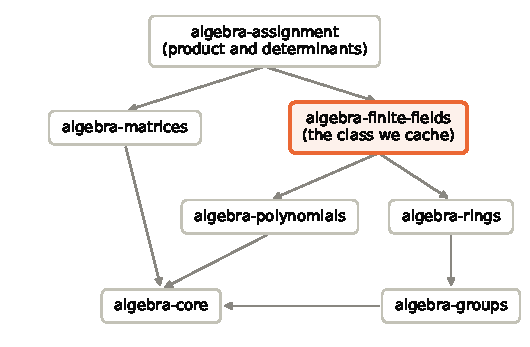
\includegraphics[width=\columnwidth]{figures/dependencies.pdf}
  \caption{The dependency chain. An arrow points from a repository to one it depends on.
  Everything below \code{algebra-finite-fields} is reached only through the finite field
  class.}
  \label{fig:dependencies}
\end{figure}

The layers are written for clarity, not speed, and the costs multiply. One field
multiplication multiplies two polynomials, which is up to nine coefficient products. Each
coefficient product is carried out by repeated addition. The product polynomial is then
divided by the modulus to get the remainder. Every intermediate polynomial is a
\code{std::vector} allocated on the heap.

\subsection{The workload}

The matrix product performs $N^3$ field multiplications and $N^3$ additions. Each
determinant is a Gaussian elimination with about $N^3/3$ multiplications, negations and
additions. In total the program asks for about $5N^3$ field operations, which is
$3.2 \times 10^{11}$ for $N = 4000$. The operands of all of them come from only 1331
values, so a binary operation has only $1331^2 = 1\,771\,561$ distinct inputs. Each one is
therefore recomputed tens of thousands of times, which is the situation caching is for.

\section{Where the original program spends its time}
\label{sec:profiling}

We profiled the original program with Callgrind, the call-graph profiler of
Valgrind~\cite{nethercote2007valgrind}, at $N = 60$. Callgrind counts executed instructions,
so the result does not depend on how fast the machine is or on what else is running.
Fig.~\ref{fig:profile} groups the instructions by the routine they were executed in.

\begin{figure}[t]
  \centering
  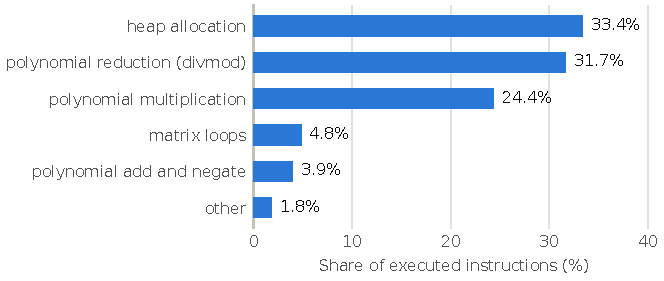
\includegraphics[width=\columnwidth]{figures/profile_original.pdf}
  \caption{Instructions executed by the original program at $N = 60$, by routine.}
  \label{fig:profile}
\end{figure}

Reducing a polynomial modulo the modulus takes \ProfileReduction\% of the instructions,
allocating and freeing the vectors that hold polynomials takes \ProfileHeap\%, and
multiplying polynomials takes \ProfileMultiply\%. The loops of the matrix product and of the
elimination themselves account for \ProfileMatrix\%. Altogether \ProfileField\% of the
instructions belong to the finite field elements: their arithmetic and the memory it
allocates.

Timing single operations gives the same picture. On our test machine one field
multiplication with the original library takes about \LookupOriginalMultiply~ns and one
addition about \LookupOriginalAdd~ns.

Every one of those instructions is reached through four member functions of the finite
field element class: \code{add}, \code{negate}, \code{multiply} and \code{reciprocal}. That
class is the narrowest point in Fig.~\ref{fig:dependencies}. Caching there leaves the matrix
library and the program untouched, and it leaves the polynomial, ring and group libraries
untouched as well, because they are only called when the cache has no answer yet. This is
why we chose the finite field class.

\section{The cached finite field}
\label{sec:cached}

\subsection{Representation and tables}

The original element stores a polynomial. The cached element stores a 16-bit index, the
position of the element in the numbering the library already defines for
\code{from\_index}: for coefficients $c_0, c_1, c_2$ the index is $c_0 + 11c_1 + 121c_2$.
Zero is index 0.

Each operation has a table. Addition and multiplication have one slot per ordered pair of
operands, $q^2$ slots each for a field of $q$ elements. Negation and reciprocal have $q$
slots each. A slot holds 0 until its result is known and the index of the result plus one
afterwards. Listing~\ref{lst:lookup} shows a multiplication.

\begin{lstlisting}[caption={A cached multiplication, simplified. \code{order} is $q$.},label={lst:lookup}]
index_type multiply(index_type a, index_type b) {
  index_type slot = products_[a * order + b];
  if (slot != 0) {
    return slot - 1;           // cache hit
  }
  return multiply_miss(a, b);  // cache miss
}
\end{lstlisting}

On a miss the library takes the two original elements from a list of all $q$ of them,
runs the original \code{multiply}, converts the result to its index, stores it, and returns
it. Each slot is filled at most once, so the four original operations run at most
$2q^2 + 2q$ times in the life of the program, however large the matrices are. Building an
element from a polynomial or an integer is not cached. It calls the original constructor,
which reduces the polynomial, and keeps the index of the result.

The tables are static arrays. They start out as zeros, so there is nothing to initialize,
and the operating system only assigns memory to the pages that are written. For $q = 1331$
they occupy 7.1~MB. The slots are atomic, so several threads can use the field at once:
two threads that miss on the same slot compute the same value and store the same value.

\subsection{A drop-in replacement}

The assignment asks that callers be able to switch implementation by changing the
dependency in CMake. We made three changes to a copy of \code{algebra-finite-fields}.
\begin{itemize}
  \item The original header \code{finite\_field.hpp} was renamed to
        \code{uncached\_finite\_field.hpp}. Its only edit is one line: the namespace changes
        from \code{algebra} to \code{algebra::uncached}. The original arithmetic is otherwise
        untouched and still compiled.
  \item A new \code{finite\_field.hpp} defines the classes \code{FiniteField} and
        \code{FiniteFieldElement} in the namespace \code{algebra}, with the same public
        members as before. They hold the index and the tables, and on a miss they call the
        original classes. \code{modulus()} returns the original class's modulus, so both
        describe the same field.
  \item A new test file compares the two (Section~\ref{sec:equivalence}).
\end{itemize}
The prime field, the modulus search, the element enumeration and the build files are
unchanged, and so is the CMake target name. In the assignment repository the switch is the
repository and tag lines of Listing~\ref{lst:switch}, in \code{cmake/Dependencies.cmake}.
No source file of the program or of the matrix library changes.

\begin{lstlisting}[language={},caption={The dependency entry that selects the
library.},label={lst:switch}]
FetchContent_Declare(
  algebra_finite_fields
  GIT_REPOSITORY git@github.com:Jplangdon/algebra-finite-fields-cached.git
  GIT_TAG        cached-v1
)
\end{lstlisting}

Fields with more than 4096 elements are not cached, because the pair tables grow with
$q^2$. Their elements hold the original element and forward every call to it, so the class
remains a correct replacement for any field the original supports.

\subsection{Why tables and not a hash map}

The assignment text suggests \code{std::unordered\_map} keyed by the operands. We measured
that option against the tables on the same stream of random operands, after filling both
caches. Fig.~\ref{fig:lookup} shows the cost per operation.

\begin{figure}[t]
  \centering
  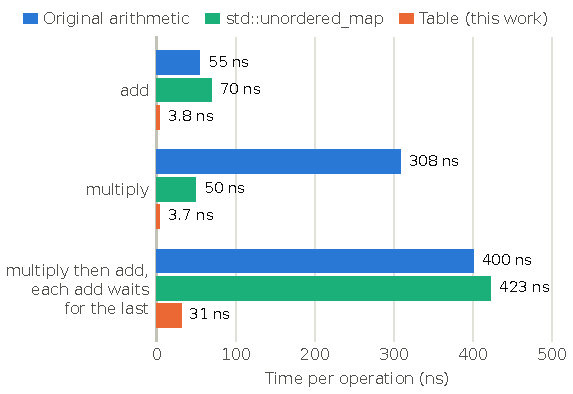
\includegraphics[width=\columnwidth]{figures/lookup_cost.pdf}
  \caption{Cost of one field operation with the original arithmetic, with a filled
  \code{std::unordered\_map} and with the filled tables.}
  \label{fig:lookup}
\end{figure}

For independent operations the hash map brings a multiplication from
\LookupOriginalMultiply~ns to \LookupMapMultiply~ns, and the table brings it to
\LookupTableMultiply~ns. The third group in the figure is the inner loop of a matrix
product, $s \leftarrow s + a_k b_k$, where each addition needs the previous sum before it can
start. \LookupChainedMapSentence. The table needs \LookupTableChained~ns, which is
\LookupChainedTableGain~times faster than the original.

The reason is memory. A hash map with 1.77 million entries keeps every entry in its own
heap node, and one lookup reads a bucket and then at least one node, each read waiting for
the one before~\cite{drepper2007memory}. A table lookup is one read from an array of
3.5~MB. Since every element is an integer below 1331, the pair of operands is already a
perfect array index and there is nothing to hash.

\section{Showing that the results are the same}
\label{sec:equivalence}

Because the field has only 1331 elements, the comparison with the original does not have to
rely on samples. The tests fall into four groups.

\textbf{The original test suite, unchanged.} The library's own test file is compiled
against the cached classes without edits and its 11 tests pass.

\textbf{Every element and every pair.} A new test file builds each element in both
implementations and compares the stored polynomial, the coefficients, the printed form and
the zero and one predicates. It then compares \code{add} and \code{multiply} on all
1\,771\,561 ordered pairs, and \code{negate} and \code{reciprocal} on all elements. Each
comparison is made twice: the first pass is answered by cache misses and the second by cache
hits, so both paths are checked. After the two passes the tests confirm that every slot that
can hold a result is filled. The reciprocal of zero has to throw the same exception in both.

\textbf{The rest of the interface.} Further tests cover the arithmetic operators,
construction from integers, coefficient lists and polynomials of degree up to 8, concurrent
use from four threads, and a field of 8192 elements that bypasses the tables.

\textbf{The assignment's computation.} One test runs the matrix product and the elimination
on $40 \times 40$ matrices in both implementations and compares the three determinants.
Beyond the unit tests, the determinants printed by the assignment program built against each
library were \SeqIdenticalVerdict{} for $N = $~\SeqIdenticalSizes.

\LibraryChecksParagraph

\section{Run time and memory before and after}
\label{sec:sequential}

\subsection{Method}

Table~\ref{tab:environments} lists the machines the measurements in this report come from.
The sequential measurements were taken on \SequentialMachine. For each matrix size the
assignment program was built twice from the same source, once against the original library
and once against the cached one, and run on one core. A small launcher starts the program
and reads its wall-clock time and its peak resident memory from the operating system when
it exits. The identity $\det(C) = \det(A)\det(B)$ was verified by the program in every run.
Every table and figure in this report is generated from the recorded result files by a
script in the repository.

\begin{table}[t]
  \caption{Machines used for the measurements.}
  \label{tab:environments}
  \centering
  \footnotesize
  \begin{tabular}{@{}l p{3.0cm} p{3.6cm}@{}}
\toprule
Label & Processor and memory & Software \\
\midrule
cloud-vm & Intel Xeon Processor @ 2.10GHz, 2 CPUs, 7.8 GiB & Ubuntu 24.04.5 LTS (virtual machine); GCC 13.3.0; Open MPI 4.1.6 \\
\bottomrule
\end{tabular}

\end{table}

\subsection{Results}

Table~\ref{tab:sequential} and Fig.~\ref{fig:runtime} give the run times. At
$N = \SeqLargestBoth$, the largest size we ran with both libraries, the original takes
\SeqOriginalAtLargest{} and the cached version \SeqCachedAtLargest, a factor of
\SeqSpeedupAtLargest. The largest cached run, $N = \SeqLargestCached$, takes
\SeqCachedAtLargestCached.

Table~\ref{tab:machines} gives the same comparison for every machine the program was run on, at the largest size each of them ran with both libraries.

\begin{table}[t]
  \caption{Original and cached finite field on each machine.}
  \label{tab:machines}
  \centering
  \footnotesize
  \setlength{\tabcolsep}{4pt}
\begin{tabular}{@{}l r r r r r r@{}}
\toprule
& & \multicolumn{3}{c}{Run time (s)} & \multicolumn{2}{c}{Memory (MiB)} \\
\cmidrule(lr){3-5}\cmidrule(l){6-7}
Machine & $N$ & Original & Cached & Speedup & Original & Cached \\
\midrule
cloud-vm & 1000 & 819 & 37.6 & 21.8$\times$ & 217 & 18.4 \\
lemmen & 1000 & 378 & 15.3 & 24.7$\times$ & 218 & 18.6 \\
\bottomrule
\end{tabular}
\end{table}


\begin{table}[t]
  \caption{The assignment program with the original and the cached finite field on
  \SequentialMachine. A dash marks a size that was not run. Where a size was run more than
  once, the median is given.}
  \label{tab:sequential}
  \centering
  \footnotesize
  \begin{tabular}{@{}r r r r r r@{}}
\toprule
& \multicolumn{3}{c}{Run time (s)} & \multicolumn{2}{c}{Peak memory (MiB)} \\
\cmidrule(lr){2-4}\cmidrule(l){5-6}
$N$ & Original & Cached & Speedup & Original & Cached \\
\midrule
100 & 0.374 & 0.295 & 1.3$\times$ & 6.2 & 11.4 \\
200 & 2.91 & 0.514 & 5.7$\times$ & 12.7 & 11.5 \\
400 & 23.5 & 1.25 & 18.8$\times$ & 38.3 & 12.2 \\
800 & 190 & 7.60 & 25.0$\times$ & 141 & 15.8 \\
1000 & 378 & 15.3 & 24.7$\times$ & 218 & 18.6 \\
2000 & -- & 147 & -- & -- & 41.2 \\
4000 & -- & 1\,182 & -- & -- & 133 \\
\bottomrule
\end{tabular}

\end{table}

\begin{figure}[t]
  \centering
  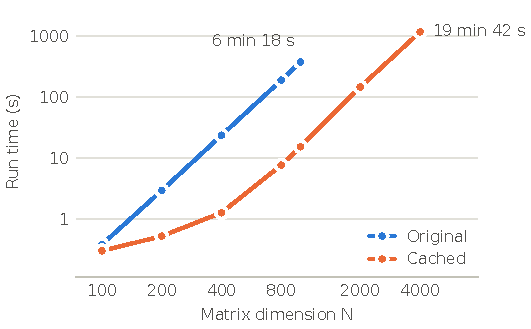
\includegraphics[width=\columnwidth]{figures/runtime.pdf}
  \caption{Run time of the whole program against matrix dimension, on logarithmic axes.}
  \label{fig:runtime}
\end{figure}

The gain grows with the matrix (Fig.~\ref{fig:speedup}), and
\SeqSmallestSentence. The reason is the first use of each operand pair.
Fig.~\ref{fig:cache} shows how the tables fill. At $N = 100$ only
\CacheHitAtHundred\% of the additions and multiplications are answered from a table, and the
rest still run the original arithmetic once. The share passes 99\% at
$N = \CacheHitNinetyNineSize$.

\begin{figure}[t]
  \centering
  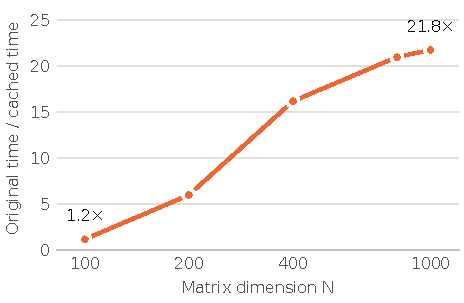
\includegraphics[width=\columnwidth]{figures/speedup.pdf}
  \caption{Speedup of the cached program over the original.}
  \label{fig:speedup}
\end{figure}

\begin{figure}[t]
  \centering
  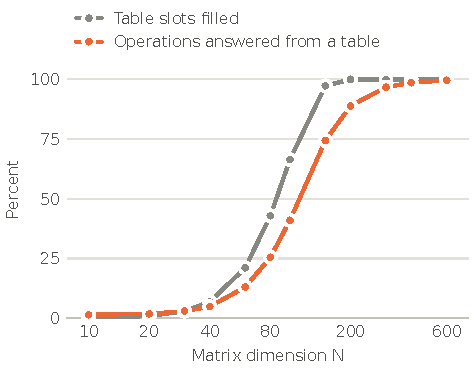
\includegraphics[width=\columnwidth]{figures/cache_fill.pdf}
  \caption{Cache behaviour over one run of the program: the share of the addition and
  multiplication table slots that end up filled, and the share of additions and
  multiplications answered from a table.}
  \label{fig:cache}
\end{figure}

\subsection{Memory}

The original library stores every matrix entry as a vector object that points to a
separate heap block. Measured from the growth of peak memory with $N$, that costs about
\SeqOriginalBytesPerEntry~bytes per entry on this system. The cached entry is two bytes.
Fig.~\ref{fig:memory} shows the effect. At $N = \SeqLargestBoth$ peak memory falls from
\SeqOriginalMemoryAtLargest{} to \SeqCachedMemoryAtLargest. The tables are a fixed cost of
about 7~MB. \SeqMemoryCrossoverSentence. At $N = \SeqLargestCached$ the cached program peaks
at \SeqCachedMemoryAtLargestCached.

\begin{figure}[t]
  \centering
  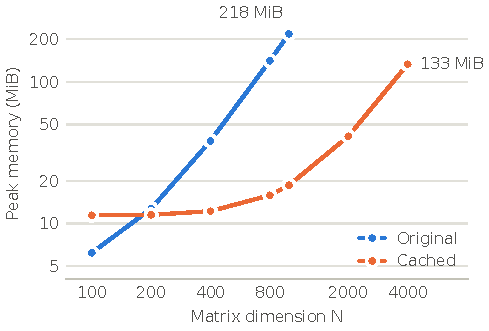
\includegraphics[width=\columnwidth]{figures/memory.pdf}
  \caption{Peak resident memory against matrix dimension, on logarithmic axes.}
  \label{fig:memory}
\end{figure}

\subsection{Where the remaining time goes}

Table~\ref{tab:phases} splits the largest run of each library into the matrix product and
the three determinants. With the cached library the product takes \SeqCachedProductShare\%
of the run, against \SeqOriginalProductShare\% with the original. The product accumulates each entry as a running
sum, so every table lookup for an addition has to wait for the previous one, which is the
chained pattern of Fig.~\ref{fig:lookup}. In the elimination the additions do not depend on
each other and the processor overlaps them.

\begin{table}[t]
  \caption{Time in the matrix product and in the three determinants, for the largest run
  of each library.}
  \label{tab:phases}
  \centering
  \footnotesize
  \begin{tabular}{@{}l r r r r@{}}
\toprule
Library & $N$ & Product (s) & Three det. (s) & Product share \\
\midrule
Original & 1000 & 425 & 393 & 52\% \\
Cached & 4000 & 2\,280 & 345 & 87\% \\
\bottomrule
\end{tabular}

\end{table}

\subsection{Comparison with the assignment's figures}

Table~\ref{tab:reference} sets our measurements beside the figures in the assignment text,
which come from a different machine. \SeqReferenceNote

\begin{table}[t]
  \caption{The assignment's reference figures (Apple M3 Max) and our measurements on
  \SequentialMachine.}
  \label{tab:reference}
  \centering
  \footnotesize
  \begin{tabular}{@{}r l r r r r@{}}
\toprule
& & \multicolumn{2}{c}{Assignment text} & \multicolumn{2}{c}{Measured here} \\
\cmidrule(lr){3-4}\cmidrule(l){5-6}
$N$ & Library & Time & Memory & Time & Memory \\
\midrule
4000 & Original & 6 h 40 min & 2.6 GB & -- & -- \\
4000 & Cached & 20 min 16 s & 0.53 GB & 43 min 48 s & 0.13 GiB \\
6000 & Original & 22 h 30 min & 5.8 GB & -- & -- \\
6000 & Cached & 1 h 08 min & 1.2 GB & -- & -- \\
\bottomrule
\end{tabular}

\end{table}

\section{An MPI determinant}
\label{sec:mpidesign}

The second part of the assignment computes the determinants with MPI~\cite{mpi40} on
several machines and compares the result with the cached sequential program.

\subsection{The elimination as a PLU factorization}

Gaussian elimination with row exchanges factors a matrix as
$PA = LU$~\cite{golub2013matrix}. At step $k$ it picks a nonzero pivot in column $k$, swaps
its row into place, divides the entries below the pivot by it to get the multipliers
$\ell_{ik}$, and subtracts $\ell_{ik}$ times row $k$ from every row $i$ below. The
determinant is the product of the pivots, with the sign flipped once for every row
exchange. If a column has no nonzero entry at or below the diagonal, the determinant is
zero. Over a finite field there is no rounding, so any nonzero entry is as good a pivot as
any other, and we take the first one.

\subsection{Distributing by columns}

The assignment text asks us to watch how pivot selection and matrix updates affect network
communication. Step $k$ needs two things: the pivot, and the multipliers below it. Both are
in column $k$. We therefore give every process whole columns, so that the process that owns
column $k$ can find the pivot and compute the multipliers from its own memory, without
asking anyone. It then tells the others the pivot row and the multipliers, and each process
updates the columns it owns: for a column $j$ it swaps the two rows, reads $x = a_{kj}$, and
computes $a_{ij} \leftarrow a_{ij} - \ell_{ik}\,x$ for the rows below.

The alternative is to distribute rows. Then the entries of column $k$ are spread over all
processes. Finding a nonzero pivot in general takes a reduction over all of them at every
step, and a row exchange can mean two processes trading rows. With columns, a row exchange
is something every process does locally to its own columns once it knows the pivot row.

\subsection{Panels}

Sending one message per column would cost $N$ broadcasts. We group $b$ neighbouring columns
into a panel and deal the panels out to the $p$ processes in turn, a one-dimensional form
of the block-cyclic layout used by ScaLAPACK~\cite{blackford1997scalapack}. Dealing them in turn keeps the load even,
because every process still owns columns near the end of the matrix. The owner of a panel
works through its $b$ columns one at a time. For each it applies the earlier steps of the
same panel, finds the pivot and computes the multipliers. It then broadcasts the whole
panel at once: a flag for a zero determinant, the $b$ pivot rows and the $b$ columns of
multipliers. Listing~\ref{lst:apply} is the routine every process runs on each of its
remaining columns.

\begin{lstlisting}[caption={Applying one panel to one column. \code{first} is the panel's
first column.},label={lst:apply}]
for (step = 0; step < steps; ++step) {
  k = first + step;
  if (pivots[step] != k)
    swap(column[k], column[pivots[step]]);
  x = column[k];
  if (x.is_zero()) continue;
  m = multipliers + step * rows;
  for (i = k + 1; i < n; ++i)
    column[i] = column[i].add(
      x.multiply(m[i - first]).negate());
}
\end{lstlisting}

The inner loop performs the same three field operations per entry as the sequential
program: a multiplication, a negation and an addition. The steps of a panel are applied to
a column one after another, in order, which gives the same result as the row-by-row
elimination.

\subsection{What travels over the network}

Rank~0 generates the matrix and sends each process its columns once. After that the only
messages are the panel broadcasts, $\lceil N/b \rceil$ of them. Together they carry each
multiplier once, about $N^2/2$ field elements whatever the value of $b$, so $b$ trades the
number of messages against their size and against the time the other processes wait while
one process prepares a panel.

The cached field matters here as well. A cached element is a plain 16-bit value, so a
column or a panel is sent as raw bytes, two per element. An element of the original library
owns heap memory and would have to be packed and unpacked. Every process keeps its own
tables. Before timing, each process fills them, which took \CacheWarmSeconds~s per process
on \MpiMachine.

\subsection{Checking the MPI program}

In every run rank~0 also computes the determinant with the sequential elimination on the
same matrix, and the program exits with an error if the two results differ. A test script
runs \MpiTestCount{} configurations, \MpiTestVerdict. They cover one to four processes,
panel widths that do and do not divide $N$, matrices smaller than the number of processes,
sparse matrices, permutation matrices and matrices with a zero leading column, which force
row exchanges, and singular matrices. For $N = 100$, 200 and 400 the script also compares
the results with the determinants printed by the original assignment program.

\section{MPI against the cached sequential program}
\label{sec:mpiresults}

\subsection{Method}

The MPI measurements were taken on \MpiMachine{} (Table~\ref{tab:environments}).
\MpiNodesSentence.

We tested $N = $~\MpiSizes{} with \MpiProcessCounts{} processes and a panel width of
$b = \MpiBlock$. The matrices are the assignment program's $A$ and $B$ for each size, built
from the same seed. \MpiRepeatsSentence, and we report medians. The MPI time runs from the
moment rank~0 starts handing out columns until rank~0 knows the determinant, so it includes
distributing the matrix. The sequential time is the assignment's elimination on the same
matrix, run by rank~0 in the same job while the other processes sleep. The two take turns
going first from one repetition to the next. Both work on the same matrix, so whichever
runs second finds the processor's caches warmed by the first, and for small matrices that
decides which one looks faster. In every measurement the MPI result and the sequential
result \MpiAllMatch.

\subsection{Break-even}

Table~\ref{tab:mpi} gives the times and Fig.~\ref{fig:mpispeedup} the ratio between them.
\MpiBreakEvenSentence. \MpiWinsSentence{} The best ratio we
measured is \MpiBestRatio{} at $N = \MpiBestRatioSize$.

\begin{table}[t]
  \caption{Median time for one determinant: the cached sequential program and the MPI
  program with $p$ processes. Each run times both on the same matrix, and the ratio is the
  median over the runs of sequential time divided by MPI time. Bold marks sizes at which MPI
  is faster.}
  \label{tab:mpi}
  \centering
  \footnotesize
  \setlength{\tabcolsep}{4pt}
  \begin{tabular}{@{}r r r r r r@{}}
\toprule
$N$ & Seq. & $p=1$ & ratio & $p=2$ & ratio \\
\midrule
10 & 1.25 $\mu$s & 1.83 $\mu$s & 0.64 & 6.00 $\mu$s & 0.32 \\
20 & 8.75 $\mu$s & 9.58 $\mu$s & 0.98 & 16.6 $\mu$s & 0.68 \\
30 & 32.5 $\mu$s & 30.6 $\mu$s & \textbf{1.04} & 41.9 $\mu$s & 0.89 \\
40 & 147 $\mu$s & 111 $\mu$s & \textbf{1.12} & 140 $\mu$s & \textbf{1.30} \\
50 & 303 $\mu$s & 250 $\mu$s & \textbf{1.17} & 261 $\mu$s & \textbf{1.26} \\
75 & 933 $\mu$s & 793 $\mu$s & \textbf{1.11} & 645 $\mu$s & \textbf{1.58} \\
100 & 1.89 ms & 1.72 ms & \textbf{1.08} & 1.02 ms & \textbf{1.78} \\
150 & 6.52 ms & 6.33 ms & \textbf{1.11} & 3.43 ms & \textbf{1.77} \\
200 & 14.1 ms & 13.1 ms & \textbf{1.15} & 7.53 ms & \textbf{1.80} \\
300 & 44.6 ms & 41.8 ms & \textbf{1.12} & 24.0 ms & \textbf{1.87} \\
400 & 100 ms & 94.3 ms & \textbf{1.09} & 53.1 ms & \textbf{1.97} \\
600 & 333 ms & 302 ms & \textbf{1.11} & 156 ms & \textbf{2.05} \\
800 & 759 ms & 738 ms & \textbf{1.07} & 418 ms & \textbf{2.02} \\
1000 & 1.47 s & 1.35 s & \textbf{1.09} & 735 ms & \textbf{2.15} \\
1500 & 4.88 s & 4.72 s & \textbf{1.02} & 2.42 s & \textbf{2.03} \\
2000 & 11.4 s & 11.3 s & \textbf{1.03} & 5.74 s & \textbf{1.99} \\
\bottomrule
\end{tabular}

\end{table}

\begin{figure}[t]
  \centering
  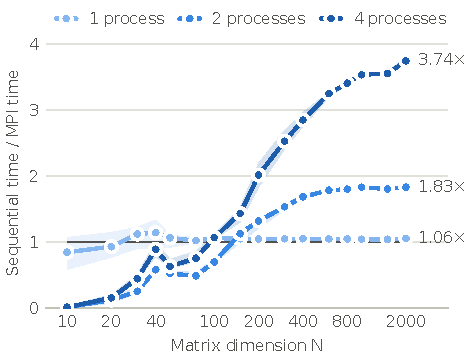
\includegraphics[width=\columnwidth]{figures/mpi_speedup.pdf}
  \caption{Sequential time divided by MPI time. Above the dark line at 1 MPI is faster.
  Each point is the median of the individual runs and the shaded band holds the middle half
  of them.}
  \label{fig:mpispeedup}
\end{figure}

For small matrices the fixed costs dominate. At the smallest sizes the arithmetic of a
determinant takes microseconds, less than it costs to hand the columns out and to send one
broadcast per panel. As $N$ grows, the arithmetic grows with $N^3$ while the number of
broadcasts grows with $N$ and their total size with $N^2$, so the messages matter less and
less.

The ratio could mix two effects, because the MPI program with a single process is not
the same code as the sequential program. It sends nothing, but it stores the matrix by
columns and eliminates one column at a time, where the assignment's elimination works row
by row. \MpiOneProcessSentence{} \MpiOneProcessWidthSentence{} The gain that comes from
the additional processes is the time with one process divided by the time with
\MpiMostProcesses, which is \MpiParallelGain{} at the largest size.

\subsection{Messages}

At $N = \MpiLargestSize$ with \MpiMostProcesses{} processes the run distributes
\MpiLargestDistributedMegabytes~MB of columns and then sends \MpiLargestPanels{} broadcasts
of \MpiLargestBroadcastMegabytes~MB in total.

\MpiBlockSentence{} That is the shape to expect. A panel that is wide compared with the
matrix leaves one process preparing most of the columns while the others wait, and a width
of one sends a broadcast for every column.

\begin{table}[t]
  \caption{Sequential time divided by MPI time for different panel widths $b$, with
  \MpiBlockProcesses{} processes. Higher is better. Bold marks the best width for each size.}
  \label{tab:blocks}
  \centering
  \footnotesize
  \begin{tabular}{@{}r r r r r r@{}}
\toprule
$N$ & $b=1$ & $b=4$ & $b=8$ & $b=32$ & $b=128$ \\
\midrule
100 & 0.30 & 0.83 & \textbf{1.07} & 0.81 & 1.01 \\
200 & 0.77 & 1.53 & \textbf{2.02} & 1.69 & 0.83 \\
400 & 1.75 & 2.68 & \textbf{2.85} & 2.54 & 1.29 \\
800 & 2.88 & 3.35 & \textbf{3.41} & 3.13 & 2.05 \\
1000 & 3.04 & 3.42 & \textbf{3.54} & 3.23 & 2.28 \\
\bottomrule
\end{tabular}

\end{table}

\section{Limitations}
\label{sec:limitations}

\textbf{Measurements.} The sequential times in Table~\ref{tab:sequential} come from one
machine, with \SeqRunsPhrase. \SeqRepeatSentence{} Small differences between neighbouring
rows therefore carry no meaning. The conclusions rest on ratios far larger than that.
\MpiNoiseSentence

\textbf{The tables and the processor's caches.} The two pair tables are 3.5~MB each. Whether
they fit in a core's cache decides how long a lookup takes, above all in the matrix product,
where the additions wait for each other. The speedup therefore depends on the processor, and
the figures here should not be read as what another machine will show.

\textbf{The sequential reference in the MPI comparison.} The MPI program times the
assignment's elimination on an array whose size is chosen at run time, so that one binary
can sweep all sizes. The assignment program fixes $N$ at compile time and checks every
index. \MpiReferenceSentence

\textbf{Where the MPI processes ran.} \MpiNodesLimitation

\textbf{Scope of the cache.} The tables need about $4q^2$ bytes, which is why fields above 4096
elements are forwarded to the original arithmetic. Constructing elements is not cached. The
matrix product is still sequential and is now the largest part of the program's run time.

\section{Conclusion}
\label{sec:conclusion}

The original program spends its instructions in the libraries underneath the finite field
class and on the memory their polynomials are kept in, and it repeats the same 1.77 million
calculations. Replacing the finite field class with a table-backed class of
the same name removed that work without touching the matrix library or the program, and
exhaustive tests show that the two classes return the same results. On \SequentialMachine{}
the $N = \SeqLargestBoth$ run became \SeqSpeedupAtLargest~times faster and its peak memory
\SeqMemoryRatioAtLargest~times smaller.

A hash map keyed by the operands, the first choice the assignment text suggests, was not
enough: \LookupConclusionPhrase, because its lookups wait on memory. An array indexed by the
two operands does not have that problem.

For the determinant, distributing columns makes pivot selection a local decision and
reduces the communication to one broadcast per panel. \MpiConclusionSentence.


\bibliographystyle{IEEEtran}
\bibliography{references}

\end{document}
